\section{Application of Shielding Techniques in TEM Cells}\label{sec:shielding-sim}
\subsection{ASTM ES7-83 method}\label{sec:astm-sim}
\FloatBarrier

\begin{figure}[htbp]
	\centering
	\includegraphics[width=1\linewidth]{content/img/se}
	\caption{Shielding effectiveness of a sheet of zinc and nickel versus the material thickness determined with the ASTM ES7-83 Method.}
	\label{fig:se}
\end{figure}

A model as described in \autoref{sec:astm} is used to determine the shielding effectiveness of barium titanate and ferrite according to the ASTM ES7-83 method discussed in \cref{sec:astm}. The TEM cell contains a shielding material sheet with a thickness of 10\,µm in the center of the TEM cell at $z=0$, which is modeled with impedance boundary conditions as discussed in \cref{sec:bc-shield}. A reference power of $P_\mathrm{ref}=1\,\mathrm{W}$ is chosen and the load power $P_\mathrm{load}$ is numerically derived. \autoref{eqn:SE_power} yields the shielding effectiveness $SE_\mathrm{dB}$ of the material depending on frequency. The investigated frequency is 1\,GHz.

%\todo[inline]{Compare results with other papers}

The properties of the materials used are listed in \autoref{tab:materials}. Ferrite additionally is modeled to have a magnetic loss tangent of $\tan \delta_m = 0.05$.

%Metallic thin shields are normally removed from the computational domain and replaced by impedance network boundary conditions on the surfaces of the shielding material \cite{1430946}. Alternatively, the inside of the shielding material contains a fine mesh created with the adaptive meshing algorithm discussed in \cref{sec:simulations}, which is applied to these simulation models. 

\begin{table}[h]
	\centering

	{\renewcommand{\arraystretch}{1.2}
		\setlength{\tabcolsep}{12pt}
		\begin{tabular}{|l|c|c|c|}
			\hline
			Material & Rel. permittivity $\varepsilon_r$ & Rel. permeability $\mu_r$ & Conductivity $\sigma$ \\
			\hline\hline
			Ferrite & $\approx 12$ & $\approx 1,000$ & $0.01$\,S/m\\
			\hline
			Barium titanate & $\approx 2,000$ & $\approx 1$ & $3.64\cdot 10^{-11}$\,S/m \\
			\hline
	\end{tabular}}
	\caption{Electromagnetic Properties of barium titanate and ferrite}
	\label{tab:materials}
\end{table}

\FloatBarrier
\subsection{Dual TEM cell}

A simulation model of two TEM cells as shown in \autoref{fig:dual_tem_cell}, consisting of the models demonstrated in \cref{sec:tem_cell_model}, without the tapered sections, is created. An empty square aperture with a side length of $d=10\,\mathrm{mm}$ is used, which makes it electrically small up to a frequency of approximately $3\,\mathrm{GHz}$. The largest numerical error stems from insufficient mesh size in the aperture region, hence 10 to 15 mesh elements across the aperture are aimed for. The procedure described in \cref{sec:dual_tem_cell} is applied to derive the electric and magnetic shielding effectiveness of, again, ferrite and barium titanate (BaTiO\textsubscript{3}).

Port 1 excites the waveguides with a power of $1\,\mathrm{W}$. The sum  $P_\mathrm{ref,sum}$ and difference $P_\mathrm{ref,diff}$ of the powers arriving at port 3 and 4 is demonstrated in \autoref{fig:emptypowersumdiff}, which is calculated using \cite{Sreenivasiah_Chang_Ma_1981}

\begin{subequations}
\begin{equation}
	P_\mathrm{sum} = (a+b)(a+b)^*,
\end{equation}
\begin{equation}
	P_\mathrm{diff} = (a-b)(a-b)^*,
\end{equation}
\end{subequations}

where $a$ and $b$ are the amplitudes of the fields at port 3 and 4, respectively.

%Simulation model leans on measurement setup in \cite{4091811}.

%\begin{figure}[htbp]
%	\centering
%	\includegraphics[width=1\linewidth]{content/img/empty-aperture-coupling}
%	\caption{Coupling of port 1 to ports 3 and 4 with empty square aperture}
%	\label{fig:empty-aperture-coupling}
%\end{figure}

\begin{figure}[htbp]
	\centering
	\includegraphics[width=1\linewidth]{content/img/empty_power_sum_diff}
	\caption{The sum $P_\mathrm{ref,sum}$ and difference $P_\mathrm{ref,diff}$ of the reference power, measured with empty aperture and calculated with the phase information considered.}
	\label{fig:emptypowersumdiff}
\end{figure}

Materials filling the aperture have a thickness of $t=10,\upmu\mathrm{m}$. 

When investigating highly conductive materials, applying skin-depth based meshing within the material enhances simulation accuracy while reducing computational effort. This approach refines the mesh especially near the material’s surface, where rapid field variations occur. The skin depth is calculated as shown in \autoref{eqn:skin_depth} and further discussed in \cref{sec:skin_effect}. In contrast, both ferrite and barium titanate have a low conductivity, therefore, the mesh refinement of the aperture is instead achieved by setting a maximum mesh element length.

Again, the sum $P_\mathrm{ref,sum}$ and difference $P_\mathrm{ref,diff}$ of the powers at port 3 and 4 are derived and shown in \cref{fig:bariumpowersumdiff,fig:ferritepowersumdiff}, once for the aperture filled with barium titanate, and once with ferrite.

\begin{figure}[htbp]
	\centering
	\begin{subfigure}[b]{0.48\textwidth}
		\centering
		\includegraphics[width=1\linewidth]{content/img/barium_power_sum_diff}
		\caption{Barium titanate}
		\label{fig:bariumpowersumdiff}
	\end{subfigure}
	\hfill
	\begin{subfigure}[b]{0.48\textwidth}
		\centering
		\includegraphics[width=1\linewidth]{content/img/ferrite_power_sum_diff}
		\caption{Ferrite}
		\label{fig:ferritepowersumdiff}
	\end{subfigure}
	\caption{The sum $P_\mathrm{load,sum}$ and difference in output power $P_\mathrm{load,diff}$ measured at port 3 and 4 with the phase information considered.}
	\label{fig:example}
\end{figure}

Ferrite exhibits higher power transfer, indicating lower shielding effectiveness compared to barium titanate. Additionally, $P_\mathrm{load,sum}$ is low for barium titanate, suggesting high electric shielding effectiveness, as indicated by \cref{eqn:se_dual_cell_e}. The power transfer of both materials increases with frequency, which can be attributed to the low bulk conductivity and slightly decreasing permittivity at higher frequencies. The electric and magnetic shielding effectiveness for both materials are illustrated in \cref{fig:sebarium,fig:seferrite}.

\begin{figure}[htbp]
	\centering
	\begin{subfigure}[b]{0.48\textwidth}
		\centering
		\includegraphics[width=1\linewidth]{content/img/se_barium}
		\caption{Barium titanate}
		\label{fig:sebarium}
	\end{subfigure}
	\hfill
	\begin{subfigure}[b]{0.48\textwidth}
		\centering
		\includegraphics[width=1\linewidth]{content/img/se_ferrite}
		\caption{Ferrite}
		\label{fig:seferrite}
	\end{subfigure}

	\caption{The electric $SE_\mathrm{dB}^\mathrm{e}$ and magnetic $SE_\mathrm{dB}^\mathrm{m}$ shielding effectiveness derived with \cref{eqn:se_dual_cell_e,eqn:se_dual_cell_m}.}
	\label{fig:se_e_m}
\end{figure}

Barium titanate exhibits good electric shielding characteristics, but demonstrates a negative $SE_\mathrm{dB}^\mathrm{m}$ value, indicating poor magnetic shielding. Negative shield effectiveness values are possible, and occur due to interference patterns at the filled aperture, which cause $a$ and the output power at port 3 to increase \cites{4091811}[p. 63]{Jaroszewski_Thomas_Rane_2019}. Ferrite, on the other hand, demonstrates a higher magnetic shielding effectiveness $SE_\mathrm{dB}^\mathrm{m}$, but a low or negative electric shielding effectiveness $SE_\mathrm{dB}^\mathrm{e}$. 

\FloatBarrier
\subsection{Antennas in shield enclosure}

The loop and monopole antennas investigated in \cref{sec:monopole,sec:loop_sim} are shielded in a hollow enclosure, as shown in \cref{fig:loopantennaenclosure,fig:monopoleantennaenclosure}. The enclosure has a thickness of $10\,$µm, and all sides have a length of 6\,mm. 

\begin{figure}[htbp]
	\centering
	\begin{subfigure}[t]{0.48\textwidth}
		\centering
		\includegraphics[width=1\linewidth]{content/img/loop_antenna_enclosure}
		\caption{Loop antenna}
		\label{fig:loopantennaenclosure}
	\end{subfigure}
	\hfill
	\begin{subfigure}[t]{0.5\textwidth}
		\centering
		\raisebox{1.5mm}{\includegraphics[width=1\linewidth]{content/img/monopole_antenna_enclosure}}
		\caption{Monopole antenna}
		\label{fig:monopoleantennaenclosure}
	\end{subfigure}
	
	\caption{Investigated antennas placed in the TEM cell covered in a cubic, hollow enclosure.}
	\label{fig:example}
\end{figure}

\autoref{fig:ferriteenclosurepower} shows the radiated power from the antennas with and without a barium titanate enclosure. The output power of the loop antenna increases because the barium titanate enclosure capacitively loads the antenna, resulting in a decrease in resonance frequency, which leads to a more efficient operating point of the antenna in the investigated frequency range, as discussed in \cref{sec:loop_sim}. In contrast, the enclosure effectively shields against the monopole antenna’s radiation. The results are consistent with the near-field region of the monopole antenna being predominantly electric (\autoref{eqn:compl_power_inf_elec_dipole}), while that of the loop antenna is predominantly magnetic (\autoref{eqn:pr_loop}).

Similarly, \autoref{fig:ferriteenclosurepower} shows the radiated power from the antennas with and without the ferrite enclosure. In this case, the output power of the monopole antenna increases due to the ferrite enclosure inductively loading the antenna. The enclosure serves as an effective shield against the loop antenna’s radiation.

\begin{figure}[htbp]
	\centering
	\begin{subfigure}[t]{0.48\textwidth}
		\centering
		\includegraphics[width=1\linewidth]{content/img/barium_enclosure_power}
		\caption{Barium titanate}
		\label{fig:bariumenclosurepower}
	\end{subfigure}
	\hfill
	\begin{subfigure}[t]{0.48\textwidth}
		\centering
		\includegraphics[width=1\linewidth]{content/img/ferrite_enclosure_power}
		\caption{Ferrite}
		\label{fig:ferriteenclosurepower}
	\end{subfigure}
	
	\caption{Output power over frequency produced by antennas with and without enclosure.}
	\label{fig:enclosurepower}
\end{figure}

\subsection{Dipole moments in shield enclosure}

Next, the antennas in the enclosures are replaced with their equivalent dipole moments determined in \cref{sec:monopole,sec:loop_sim}. 

\FloatBarrier
%\subsection{Shielding Antennas}
%
%\todo[inline]{shielding antennas and investigating field distribution will be done here. Some tilt in shielding material would be interesting to investigate}
%
%\subsection{Shielding Equivalent Dipole Moments}
%
%\todo[inline]{Check latex comments, which contain some good ideas. TODO Rest of section}

%\todo[inline]{Rest of shielding material section still TODO}
%\subsection{Shielding effectiveness of graphite}
%
%The reference power $P_\mathrm{ref}$ has been set to 1\,W. Using \autoref{eqn:load_power} and the S-parameters from the simulation results, $P_\mathrm{load}$ may be determined. \autoref{fig:se_graphite} demonstrates the shielding effectiveness of graphite in dB $SE_\mathrm{dB}$ over the shielding material thickness. The solution frequency is 500\,MHz. A frequency sweep shows that the reflection coefficient $S_{11}$ does not depend much on the frequency. 
%
%\begin{figure}[h]
%	\centering
%	\includegraphics[width=1\linewidth]{content/img/se_graphite.png}
%	\caption{Shielding effectiveness of graphite}
%	\label{fig:se_graphite}
%\end{figure}
%
%The components of $SE_\mathrm{dB}$ are determined according to \autoref{eqn:se_rereflections}. 
%
%\subsection{Shield effectiveness of FR4}
%
%The FR4 has a relative permittivity of $\epsilon_r=4.4$. According to \autoref{eqn:rel_wave_imp}, the relative wave impedance is $Z=0.476$. This leads to a reflection coefficient of $R=-0.355$ by \autoref{eqn:reflection_coefficient_plane_dielectric}.
%
%
%The reflection coefficient $|S_{11}|=0.045$.
%
%\subsection{Dual TEM Cell}
%
%A simulation setup of a dual TEM cell is created. A rectangular aperture with a side length of $l=5\,\mathrm{cm}$, inspired by \cite{Wilson_1981}, connects both TEM cells. One waveport 1, as in \autoref{fig:dual_tem_cell}, is excited with a power of $P=1\,\mathrm{W}$. The simulation is conducted, leaving the aperture open. A second one determines the coupling of the waveports, when the aperture is filled with a graphite sheet with a thickeness of $t=50$\,µm.
%
%At a frequency of $f=500\,\mathrm{MHz}$, the coupling between waveport 1 to the waveports 3 and 4 of the receiving TEM cell is shown in \autoref{tab:dual_tem_fwd_trans}. Only one frequency point is investigated, as the results stay roughly constant over the inspected frequency range from 100\,MHz to 1\,GHz. 
%
%
%\begin{table}
%	\centering
%	\begin{tabular}{|c|c|c|}
%		\hline
%		Forward transmission coefficient & Empty aperture & aperture filled with FR408\\\hline\hline
%		Waveport 1 to 3 $S_{13}$ & -83.80\,dB, -144.96° & -85.27\,dB, -155.79°\\\hline
%		Waveport 1 to 4 $S_{14}$ & -90.31\,dB, -144.96° & -87.14\,dB, 25.00°\\\hline
%	\end{tabular}
%	\caption{Forward transmission coefficients}
%	\label{tab:dual_tem_fwd_trans}
%\end{table}
%\todo{Why -8dB difference in empty aperture? Explained in \cite{Wilson_1981}}
%
%Using \autoref{eqn:se_dual_cell_e} and \autoref{eqn:se_dual_cell_m} leads to the shielding effectiveness for electric coupling $SE_\mathrm{dB}^\mathrm{e}=19.07\,\mathrm{dB}$ and magnetic coupling $SE_\mathrm{dB}^\mathrm{m}=-9.22\,\mathrm{dB}$. \todo{negative SE possible? Redo Simulations with finer Mesh around aperture} To get the sum $P_\mathrm{sum}$ and difference $P_\mathrm{diff}$ of powers, the phase of the signals have to be considered. With unit input power at the transmitting TEM cell, \autoref{eqn:s_param_to_power_sum} and \autoref{eqn:s_param_to_power_diff} are used for this purpose \cite{Sreenivasiah_Chang_Ma_1981}. 
%
%\begin{subequations}
%	\begin{equation}
%		P_\mathrm{sum} = (S_{13} + S_{14})(S_{13} + S_{14})^*
%		\label{eqn:s_param_to_power_sum}
%	\end{equation}
%	\begin{equation}
%		P_\mathrm{diff}= (S_{13} - S_{14})(S_{13} - S_{14})^*
%		\label{eqn:s_param_to_power_diff}
%	\end{equation}
%\end{subequations}
%
%Indicated by the phase shift of roughly 180°, the coupling between the TEM cells occur mainly due to magnetic dipoles. Due to the relative permittivity of $\epsilon _\mathrm{r}=3.66$ and the relative permeability of $\mu_r\approx 1$ of the shielding material, the magnetic fields dominate. This leads to a energy transfer mainly due to magnetic dipole moments\todo{One port receives overall more power due to the material. Is it because of the magnetic/electric dipoles in it? Check mesh around the small aperture.} The overall shielding effectiveness $SE_\mathrm{dB}=$ \autoref{eqn:dual_tem_cell_tot_power}.
%
%\begin{equation}
%	P_\mathrm{total}=|S_{13}|^2+|S_{14}|^2
%	\label{eqn:dual_tem_cell_tot_power}
%\end{equation}

% Show which dipole moments are affected by an offset in z-direction, and which ones are not.
